\icode[magenta]{N21L-ME-CA-L4-261019-002}
\nceeID[16]{2021山东}{18}
如图所示，三个质量均为\(m\)的小物块\(A\)、\(B\)、\(C\)，放置在水平面上，\(A\)紧靠竖直墙壁，一劲度系数为\(k\)的轻弹簧将\(A\)、\(B\)相接，\(C\)紧靠\(B\)，开始时弹簧处于原长，\(A\)、\(B\)、\(C\)均静止。现给\(C\)施加一水平向左、大小为\(F\)的恒力，使\(B\)、\(C\)一起向左运动，当速度为0时，立即撤去恒力，一段时间后\(A\)离开墙壁，最终三物块都停止运动。已知\(A\)、\(B\)、\(C\)与地面间的滑动摩擦力大小均为\(f\)，最大静摩擦力等于滑动摩擦力，弹簧始终在弹性限度内。（弹簧的弹性势能可表示为：\(E_p = \frac{1}{2}kx^2\)，\(k\)为弹簧的劲度系数，\(x\)为弹簧的形变量）

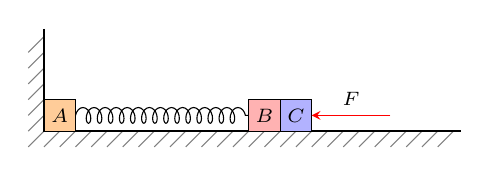
\begin{tikzpicture}[font=\scriptsize]
    \foreach \y in {-.2,0,...,1.1}
        \draw[gray] (-.2,\y)--++(.2,.2);
    \foreach \x in {0,.2,...,5.1}
        \draw[gray] (\x,-.2)--++(.2,.2);
    \draw[thick] (0,1.3)--(0,0)--(5.3,0);
    \draw[fill=orange!40] (0,0) rectangle (.4,.4)node[midway]{\(A\)};
    \draw[decoration={aspect=.6,segment length=4,amplitude=1mm,coil},decorate] (.4,.2)--(2.6,.2);
    \draw[fill=red!30] (2.6,0) rectangle (3,.4)node[midway]{\(B\)};
    \draw[fill=blue!30] (3,0) rectangle (3.4,.4)node[midway]{\(C\)};
    \draw[-stealth,red] (4.4,.2)--node[above,black]{\(F\)}(3.4,.2);
\end{tikzpicture}
\begin{enumerate}
    \item 求\(B\) 、\(C\)向左移动的最大距离\(x_0\) 和\(B\) 、\(C\)分离时\(B\)的动能\(E_k\)；
    \item 为保证\(A\)能离开墙壁，求恒力的最小值\(F_{\min}\)；
    \item 若三物块都停止时\(B\) 、\(C\)间的距离为\(x_{BC}\)，从\(B\) 、\(C\)分离到\(B\)停止运动的整个过程，\(B\)克服弹簧弹力做的功为\(W\)，通过推导比较\(W\)与\(fx_{BC}\)的大小；
    \item 若\(F = 5f\)，请在所给的坐标系中，画出\(C\)向右运动过程中加速度\(a\)随位移\(x\)变化的图像，并在坐标轴上标出开始运动和停止运动时\(a\)、\(x\)值（用\(f\)、\(k\)、\(m\)表示），不要求推导过程。以撤去\(F\)时\(C\)的位置为坐标原点，水平向右为正方向。
\end{enumerate}

